\documentclass[11pt,letterpaper]{article}
\usepackage[utf8]{inputenc}
\usepackage{amsmath}
\usepackage{amsfonts}
\usepackage{amssymb}
\usepackage[margin=1in]{geometry}
\usepackage{graphicx}
\usepackage{sidecap}
\usepackage{float}
\title{Regression with Gradient Descent\vspace{-3.5ex}}
\begin{document}
\newgeometry{top=.25in,left=1in,right=1in,bottom=1in}
\maketitle
\vspace{-3em}
\section{}
First, we discuss variations on gradient descent, including analytic gradient descent, finite difference gradient descent, and Matlab's \texttt{fminunc}, which includes some variations such as adaptive step size, using a quadratic approximation instead of linear approximation, and using a 2-dimensional subspace to reduce computational complexity. First, we'll examine the analytic gradient descent, which relies on having an analytic gradient expression at all points in space.

We'll refer to three example functions: the $n$-dimensional quadratic ``bowl'', $Q_n$, the $n$-dimensional inverted Gaussian (centered at $\mu = 0$, with $\Sigma = \mathbf I_n$), $N_n$, and the $n$-dimensional sum of $\sin$'s, $S_n$. These are defined as follows (leaving off the normalization constant on the inverted Gaussian for simplicity):

\[ Q_n = \left\| \mathbf x \right\| ^2 \]

\[ N_n = -\exp{\left(-\dfrac{1}{2} \left\| \mathbf x \right\| ^2 \right)} \]

\[ S_n = \sum_{i=1}^n \sin(x_n) \]
Next, we benchmark the gradient descent variations on these two functions (seeding with an initial guess of $(1,1,\ldots)$):

\begin{table}[h]
\centering
\caption{Iterations (step = .1, threshold = .001)}
\begin{tabular}{r|ccc|ccc|ccc}
   & \multicolumn{3}{|c}{Analytic Gradient} & \multicolumn{3}{|c}{Finite Differences} & \multicolumn{3}{|c}{\texttt{fminunc}} \\
$n$& $Q_n$         & $N_n$        & $S_n$   & $Q_n$              & $N_n$   & $S_n$           & $Q_n$         & $N_n$        & $S_n$ \\\hline
2  & 16            & 33           & 46      & 16                 & 33      & 46              & 6             & 15           & 18    \\
5  & 18            & 60           & 50      & 18                 & 60      & 50              & 12            & 48           & 36    \\
20 & 21            &  1           & 57      & 21                 &  1      & 57              & 42            & 21           & 126   \\
100& 25            &  1           & 64      & 25                 &  1      & 64              & 202           & 101          & 606   
\end{tabular}
\end{table}

Focusing on just $S_n$, and leaving the step size, starting point, and threshold the same unless otherwise noted, we may also examine the effects of each variable (defaulting to $n=5$:

\begin{table}[h]
\centering
\caption{Examining the effect of other variables}
\begin{tabular}{cc|cc|cc}
\multicolumn{2}{c}{Step Size}& \multicolumn{2}{|c}{Starting Point} & \multicolumn{2}{|c}{Threshold} \\
$\Delta$  & Iterations        & $x_0$   & Iterations   & $\delta$  & Iterations     \\\hline
2.0       & 177               & 0.001   & 49           & 0.01      & 39     \\
1.0       & 5                 & 0.01    & 49           & 0.001     & 50     \\
0.1       & 61                & 0.1     & 50           & 0.0001    & 61     \\
0.01      & 503               & 1.0     & 61           & 0.00001   & 72  
\end{tabular}
\end{table}

We notice that the finite differences and analytic methods yield the exact same number of iterations for all functions. This can be explained by examining the diagonal of the Hessian matrix for each of the functions - in all cases, the values are small, indicating low curvature, and thus that the function can be well-approximated by the linear finite difference approximation. Therefore, when examining the effects of other variables, we only present the numbers using the finite-difference gradient (the analytic gradient produces identical numbers). We may draw a few conclusions by examining the effects of other variables. As we decrease the step size, it takes longer to converge. However, increasing the step size beyond 1 causes the iteration to overshoot, resulting in an overall higher number of required iterations. Moving the starting point further from the minimum increases the number of iterations, but only slightly, because the gradient increases, which increases the step size proportionally. Finally, requiring a stricter convergence criteria via a smaller threshold increases the number of iterations, but only by a constant amount, because the gradient again ensures the step size is in proportion to the distance from the minimum.\\

By plotting the difference between the finite differences approximation, we can see the accuracy achieved. Here, we again use $\delta = .01$. Figures \ref{fig:gradDifQ} through \ref{fig:gradDifS} are plots of $(\nabla f(\mathbf{x}) - \tilde{\nabla} f(\mathbf{x}))/f(\mathbf{x})$ for $x=(0,1)$.

\begin{figure}[!htb]
\minipage{0.32\textwidth}
  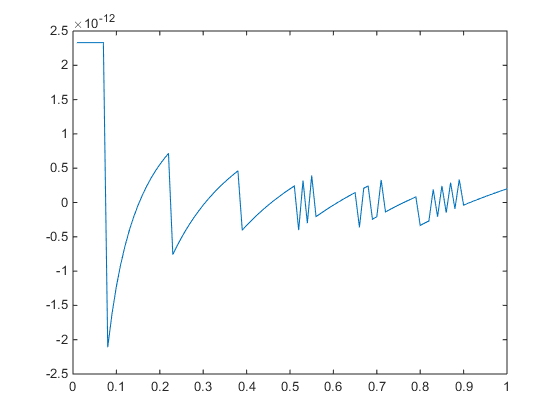
\includegraphics[width=\linewidth]{figures/gradDifQ.png}
  \caption{$Q_1$, scale of $10^{-12}$}\label{fig:gradDifQ}
\endminipage\hfill
\minipage{0.32\textwidth}
  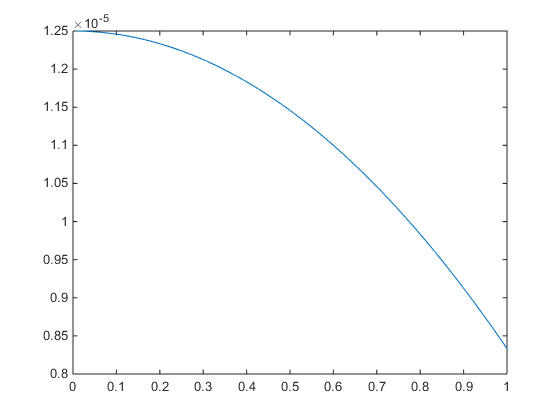
\includegraphics[width=\linewidth]{figures/gradDifN.png}
  \caption{$N_1$, scale of $10^{-5}$}\label{fig:gradDifN}
\endminipage\hfill
\minipage{0.32\textwidth}
  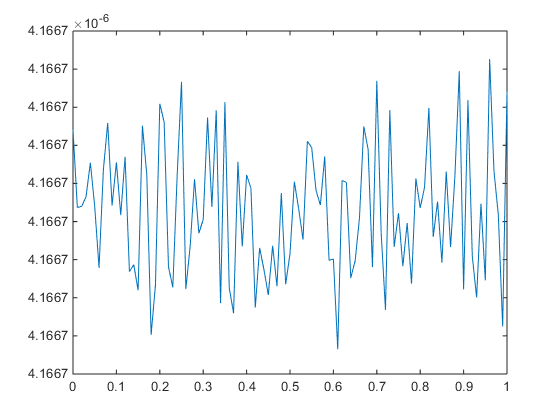
\includegraphics[width=\linewidth]{figures/gradDifS.png}
  \caption{$S_1$, scale of $10^{-6}$}\label{fig:gradDifS}
\endminipage
\end{figure}

Given the scales of the plots, it is clear that the finite differences method is quite accurate for these functions over these distance scales. As noted, this is generally true when the diagonal entries of the Hessian matrix are small.

\section{}
Another way we can benchmark our gradient descent method is to perform basis function regression on some given sample data points. Given, say, $10$ data points $X = x^{(1:10)}$ that are generated from a noisy distribution from $y = \sin(2\pi x)$, we'll try to estimate the generating function based on (a) the values at the data points $Y = y^{(1:10)}$ and (b) a basis set of functions.\\
We can begin by considering a simple polynomial basis; i.e. $\phi(x) = [1, x, x^2, \ldots , x^M]$ where $M$ is the degree of the polynomial we are considering. We wish to minimize our parameter $\theta$, which has a well-known analytic solution:
$$\theta = (\Phi^T\Phi)^{-1}\Phi^Ty$$
given that
$$\Phi = some matrix here$$
while limited to our polynomial basis. We can easily test this by plotting our data $(X, Y)$ with our learned model $\theta^T\Phi(X)$ for varying values of $M$:
We note that we can't have $M > 10$, or else we have too many parameters to adjust for the data points that we have. We can adjust for this using the \textit{Moore-Penrose inverse}, but we will not address it in detail here.\\
However, we can generalize our basis functions to more than simply polynomials in $x$. In this way, we can introduce trigonometric bases, exponential bases, etc. to give us more flexibility in choosing the parameter $\theta$. Our ultimate goal is the minimize the sum of the squared errors, or $SSE(\theta)$, equal to
$$\text{SSE}(\theta) = \sum_{i=1}^n (\theta^T\phi(x^{(i)}) - y^{(i)})^2$$.
We can minimize this by using gradient descent, which we discussed earlier. We can then confirm our calculations analytically by computing the derivative of $\text{SSE}(\theta)$:
$$\frac{\partial}{\partial\theta}\Big(\sum_{i=1}^n (\theta^T\phi(x^{(i)}) - y^{(i)})^2\Big) = 2\sum_{i=1}^n \phi(x^{(i)})(\theta^T\phi(x^{(i)}) - y^{(i)})$$
Plugging in our optimal $\theta$ into this formula, we obtain the following results for our derivative:

Now let us try minimizing the $\theta$ for our original dataset $(X, Y)$ drawn from a distribution following $y = \sin(x)$. Using gradient descent, we obtain the following results:

It is tempting, to fit this data set, to use $\phi_1(x) = \sin(2\pi x), \ldots , \phi_M(2\pi Mx)$ as our basis set of functions. If we use these, our plots look much closer to the real value:

However, if we didn't already know anything about the data, guessing a basis of sine functions comes with a serious disadvantage. It guarantees that all your generated $\theta^T\phi(x)$ will be periodic in nature, when your actual data/observations really aren't. This can cause unnecessarily varying, and potentially totally off, data to be predicted.

\section{}

Here we examine ridge regression, which is a form of regression that attempts to minimize the coefficients of $\Theta$. It does this by imposing a penalty, $\lambda$, on the Euclidean norm of the coefficients of $\Theta$. The fact that we impose a penalty on the Euclidean norm is a direct result of considering the noise as a Gaussian. Considering the noise as a Laplacian distribution leads to imposing a penalty on the absolute value norm, while other noise distributions lead to yet more functions of $\theta$ to apply the penalty to. The analytic solution to this minimization is given by
\[ \theta = (\Phi^\intercal \Phi + \lambda \mathbf{I})^{-1}\Phi^\intercal y \]
Where $\Phi = \phi(x)$. We then have the predictor function given by $\phi$ weighted by $\theta$, eg, we would predict $y_{predicted} = \theta^\intercal \phi(x')$. We can see the effect $\lambda$ has on the result by examining a few values of $\lambda$ for the same dataset used previously (generated from $\sin(2\pi x)$).
\begin{figure}[!htb]
\minipage{0.49\textwidth}
  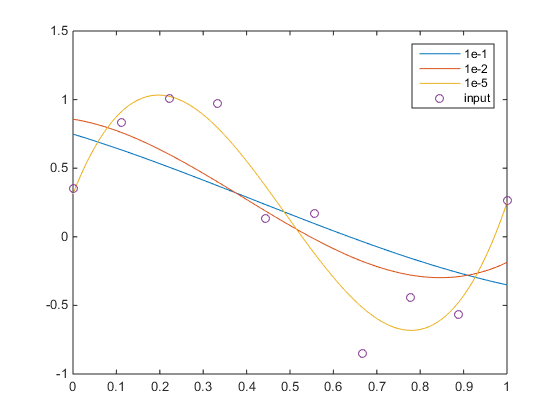
\includegraphics[width=\linewidth]{figures/M3.png}
  \caption{$M=3$}\label{fig:M3}
\endminipage\hfill
\minipage{0.49\textwidth}
  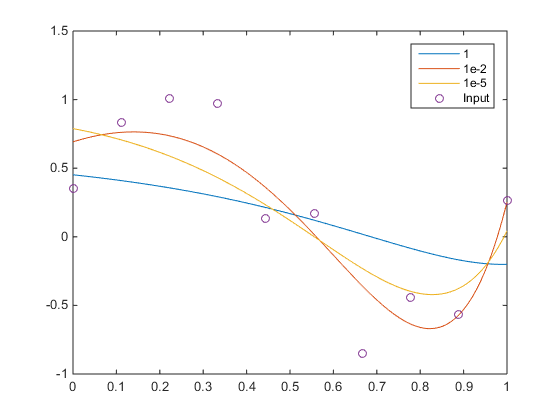
\includegraphics[width=\linewidth]{figures/M7.png}
  \caption{$M=7$}\label{fig:M7}
\endminipage
\end{figure}
The effect of $\lambda$ is clear in Figures \ref{fig:M3} and \ref{fig:M7}, where higher values of $\lambda$ lead to flatter, smoother approximations. As $M$ increases (especially relative to $n$), the values in $\theta$ begin rising enormously, but adding the $\lambda$ factor helps to keep them under control. For example, in this example with $M=7$, $\max \theta_i = 1595.9$ for $\lambda = 0$, but for $\lambda = .01$, $\max \theta_i = 1.7781$, a much more reasonable value, and far more likely to approximate the truth accurately. In particular, Figure 1.8 in Bishop nicely summarizes the assistance $\lambda$ gives in generalizing $\theta$.

\end{document}













